% Options for packages loaded elsewhere
\PassOptionsToPackage{unicode}{hyperref}
\PassOptionsToPackage{hyphens}{url}
%
\documentclass[
  ignorenonframetext,
]{beamer}
\usepackage{pgfpages}
\setbeamertemplate{caption}[numbered]
\setbeamertemplate{caption label separator}{: }
\setbeamercolor{caption name}{fg=normal text.fg}
\beamertemplatenavigationsymbolsempty
% Prevent slide breaks in the middle of a paragraph
\widowpenalties 1 10000
\raggedbottom
\setbeamertemplate{part page}{
  \centering
  \begin{beamercolorbox}[sep=16pt,center]{part title}
    \usebeamerfont{part title}\insertpart\par
  \end{beamercolorbox}
}
\setbeamertemplate{section page}{
  \centering
  \begin{beamercolorbox}[sep=12pt,center]{part title}
    \usebeamerfont{section title}\insertsection\par
  \end{beamercolorbox}
}
\setbeamertemplate{subsection page}{
  \centering
  \begin{beamercolorbox}[sep=8pt,center]{part title}
    \usebeamerfont{subsection title}\insertsubsection\par
  \end{beamercolorbox}
}
\AtBeginPart{
  \frame{\partpage}
}
\AtBeginSection{
  \ifbibliography
  \else
    \frame{\sectionpage}
  \fi
}
\AtBeginSubsection{
  \frame{\subsectionpage}
}
\usepackage{amsmath,amssymb}
\usepackage{iftex}
\ifPDFTeX
  \usepackage[T1]{fontenc}
  \usepackage[utf8]{inputenc}
  \usepackage{textcomp} % provide euro and other symbols
\else % if luatex or xetex
  \usepackage{unicode-math} % this also loads fontspec
  \defaultfontfeatures{Scale=MatchLowercase}
  \defaultfontfeatures[\rmfamily]{Ligatures=TeX,Scale=1}
\fi
\usepackage{lmodern}
\usetheme[]{Madrid}
\ifPDFTeX\else
  % xetex/luatex font selection
\fi
% Use upquote if available, for straight quotes in verbatim environments
\IfFileExists{upquote.sty}{\usepackage{upquote}}{}
\IfFileExists{microtype.sty}{% use microtype if available
  \usepackage[]{microtype}
  \UseMicrotypeSet[protrusion]{basicmath} % disable protrusion for tt fonts
}{}
\makeatletter
\@ifundefined{KOMAClassName}{% if non-KOMA class
  \IfFileExists{parskip.sty}{%
    \usepackage{parskip}
  }{% else
    \setlength{\parindent}{0pt}
    \setlength{\parskip}{6pt plus 2pt minus 1pt}}
}{% if KOMA class
  \KOMAoptions{parskip=half}}
\makeatother
\usepackage{xcolor}
\newif\ifbibliography
\usepackage{color}
\usepackage{fancyvrb}
\newcommand{\VerbBar}{|}
\newcommand{\VERB}{\Verb[commandchars=\\\{\}]}
\DefineVerbatimEnvironment{Highlighting}{Verbatim}{commandchars=\\\{\}}
% Add ',fontsize=\small' for more characters per line
\usepackage{framed}
\definecolor{shadecolor}{RGB}{248,248,248}
\newenvironment{Shaded}{\begin{snugshade}}{\end{snugshade}}
\newcommand{\AlertTok}[1]{\textcolor[rgb]{0.94,0.16,0.16}{#1}}
\newcommand{\AnnotationTok}[1]{\textcolor[rgb]{0.56,0.35,0.01}{\textbf{\textit{#1}}}}
\newcommand{\AttributeTok}[1]{\textcolor[rgb]{0.13,0.29,0.53}{#1}}
\newcommand{\BaseNTok}[1]{\textcolor[rgb]{0.00,0.00,0.81}{#1}}
\newcommand{\BuiltInTok}[1]{#1}
\newcommand{\CharTok}[1]{\textcolor[rgb]{0.31,0.60,0.02}{#1}}
\newcommand{\CommentTok}[1]{\textcolor[rgb]{0.56,0.35,0.01}{\textit{#1}}}
\newcommand{\CommentVarTok}[1]{\textcolor[rgb]{0.56,0.35,0.01}{\textbf{\textit{#1}}}}
\newcommand{\ConstantTok}[1]{\textcolor[rgb]{0.56,0.35,0.01}{#1}}
\newcommand{\ControlFlowTok}[1]{\textcolor[rgb]{0.13,0.29,0.53}{\textbf{#1}}}
\newcommand{\DataTypeTok}[1]{\textcolor[rgb]{0.13,0.29,0.53}{#1}}
\newcommand{\DecValTok}[1]{\textcolor[rgb]{0.00,0.00,0.81}{#1}}
\newcommand{\DocumentationTok}[1]{\textcolor[rgb]{0.56,0.35,0.01}{\textbf{\textit{#1}}}}
\newcommand{\ErrorTok}[1]{\textcolor[rgb]{0.64,0.00,0.00}{\textbf{#1}}}
\newcommand{\ExtensionTok}[1]{#1}
\newcommand{\FloatTok}[1]{\textcolor[rgb]{0.00,0.00,0.81}{#1}}
\newcommand{\FunctionTok}[1]{\textcolor[rgb]{0.13,0.29,0.53}{\textbf{#1}}}
\newcommand{\ImportTok}[1]{#1}
\newcommand{\InformationTok}[1]{\textcolor[rgb]{0.56,0.35,0.01}{\textbf{\textit{#1}}}}
\newcommand{\KeywordTok}[1]{\textcolor[rgb]{0.13,0.29,0.53}{\textbf{#1}}}
\newcommand{\NormalTok}[1]{#1}
\newcommand{\OperatorTok}[1]{\textcolor[rgb]{0.81,0.36,0.00}{\textbf{#1}}}
\newcommand{\OtherTok}[1]{\textcolor[rgb]{0.56,0.35,0.01}{#1}}
\newcommand{\PreprocessorTok}[1]{\textcolor[rgb]{0.56,0.35,0.01}{\textit{#1}}}
\newcommand{\RegionMarkerTok}[1]{#1}
\newcommand{\SpecialCharTok}[1]{\textcolor[rgb]{0.81,0.36,0.00}{\textbf{#1}}}
\newcommand{\SpecialStringTok}[1]{\textcolor[rgb]{0.31,0.60,0.02}{#1}}
\newcommand{\StringTok}[1]{\textcolor[rgb]{0.31,0.60,0.02}{#1}}
\newcommand{\VariableTok}[1]{\textcolor[rgb]{0.00,0.00,0.00}{#1}}
\newcommand{\VerbatimStringTok}[1]{\textcolor[rgb]{0.31,0.60,0.02}{#1}}
\newcommand{\WarningTok}[1]{\textcolor[rgb]{0.56,0.35,0.01}{\textbf{\textit{#1}}}}
\usepackage{graphicx}
\makeatletter
\def\maxwidth{\ifdim\Gin@nat@width>\linewidth\linewidth\else\Gin@nat@width\fi}
\def\maxheight{\ifdim\Gin@nat@height>\textheight\textheight\else\Gin@nat@height\fi}
\makeatother
% Scale images if necessary, so that they will not overflow the page
% margins by default, and it is still possible to overwrite the defaults
% using explicit options in \includegraphics[width, height, ...]{}
\setkeys{Gin}{width=\maxwidth,height=\maxheight,keepaspectratio}
% Set default figure placement to htbp
\makeatletter
\def\fps@figure{htbp}
\makeatother
\setlength{\emergencystretch}{3em} % prevent overfull lines
\providecommand{\tightlist}{%
  \setlength{\itemsep}{0pt}\setlength{\parskip}{0pt}}
\setcounter{secnumdepth}{-\maxdimen} % remove section numbering
\logo{
\includegraphics[height=1cm,width=3cm]{logo.png}}
\usetheme{Madrid}
\usefonttheme{serif}
\setbeamertemplate{navigation symbols}{}
\usepackage{lmodern}  % for bold teletype font
\usepackage{amsmath}  % for \hookrightarrow
\usepackage{xcolor}   % for \textcolor


\ifLuaTeX
  \usepackage{selnolig}  % disable illegal ligatures
\fi
\IfFileExists{bookmark.sty}{\usepackage{bookmark}}{\usepackage{hyperref}}
\IfFileExists{xurl.sty}{\usepackage{xurl}}{} % add URL line breaks if available
\urlstyle{same}
\hypersetup{
  pdftitle={Leksioni 5},
  pdfauthor={Endri Raco},
  hidelinks,
  pdfcreator={LaTeX via pandoc}}

\title{Leksioni 5}
\author{Endri Raco}
\date{04 May, 2024}

\begin{document}
\frame{\titlepage}

\begin{frame}[allowframebreaks]
  \tableofcontents[hideallsubsections]
\end{frame}
\hypertarget{tuxeb-dhuxebnat-raster-vazhdim}{%
\section{Të dhënat Raster
(vazhdim)}\label{tuxeb-dhuxebnat-raster-vazhdim}}

\begin{frame}[fragile]{Analiza e Pikave dhe Vlerësimi i Dendësisë së
Kernelit (KDE)}
\protect\hypertarget{analiza-e-pikave-dhe-vleruxebsimi-i-denduxebsisuxeb-suxeb-kernelit-kde}{}
\AddToHookNext{env/Highlighting/begin}{\tiny}

\begin{Shaded}
\begin{Highlighting}[]
\ImportTok{import}\NormalTok{ urllib.request}

\CommentTok{\# Shkarkoni të dhënat e anijeve të mbytura historike}
\NormalTok{url\_shipwrecks }\OperatorTok{=} \StringTok{\textquotesingle{}https://github.com/endri81/instatgis/blob/master/data/gis4/darmc\_historical\_shipwrecks\_500bce\_1500ce.geojson?raw=true\textquotesingle{}}
\NormalTok{file\_name\_shipwrecks }\OperatorTok{=} \StringTok{\textquotesingle{}data/darmc\_historical\_shipwrecks\_500bce\_1500ce.geojson\textquotesingle{}}
\NormalTok{urllib.request.urlretrieve(url\_shipwrecks, file\_name\_shipwrecks)}

\CommentTok{\# Shkarkoni gjithashtu kufijtë e vendeve}
\NormalTok{url\_boundaries }\OperatorTok{=} \StringTok{\textquotesingle{}https://github.com/endri81/instatgis/blob/master/data/gis4/natural\_earth\_world\_boundaries\_50m\_2018.geojson?raw=true\textquotesingle{}}
\NormalTok{file\_name\_boundaries }\OperatorTok{=} \StringTok{\textquotesingle{}data/natural\_earth\_world\_boundaries\_50m\_2018.geojson\textquotesingle{}}
\NormalTok{urllib.request.urlretrieve(url\_boundaries, file\_name\_boundaries)}
\end{Highlighting}
\end{Shaded}
\end{frame}

\begin{frame}[fragile]{Ngarkimi dhe Projekti i Dataset-eve}
\protect\hypertarget{ngarkimi-dhe-projekti-i-dataset-eve}{}
\AddToHookNext{env/Highlighting/begin}{\tiny}

\begin{Shaded}
\begin{Highlighting}[]
\ImportTok{import}\NormalTok{ geopandas }\ImportTok{as}\NormalTok{ gpd}

\CommentTok{\# Ngarkoni dataset{-}in dhe projektoni në 3035 (Lambert, i përshtatshëm për Evropën)}
\NormalTok{ship\_df }\OperatorTok{=}\NormalTok{ gpd.read\_file(}\StringTok{\textquotesingle{}data/darmc\_historical\_shipwrecks\_500bce\_1500ce.geojson\textquotesingle{}}\NormalTok{).to\_crs(}\DecValTok{3035}\NormalTok{)}
\NormalTok{countries\_df }\OperatorTok{=}\NormalTok{ gpd.read\_file(}\StringTok{\textquotesingle{}data/natural\_earth\_world\_boundaries\_50m\_2018.geojson\textquotesingle{}}\NormalTok{).to\_crs(}\DecValTok{3035}\NormalTok{)}
\end{Highlighting}
\end{Shaded}
\end{frame}

\begin{frame}[fragile]{Shfaqni një shembull të të dhënave}
\protect\hypertarget{shfaqni-njuxeb-shembull-tuxeb-tuxeb-dhuxebnave}{}
\AddToHookNext{env/Highlighting/begin}{\tiny}

\begin{Shaded}
\begin{Highlighting}[]
\NormalTok{ship\_df.sample(}\DecValTok{5}\NormalTok{)}
\end{Highlighting}
\end{Shaded}
\end{frame}

\begin{frame}{Shfaqni një shembull të të dhënave}
\protect\hypertarget{shfaqni-njuxeb-shembull-tuxeb-tuxeb-dhuxebnave-1}{}
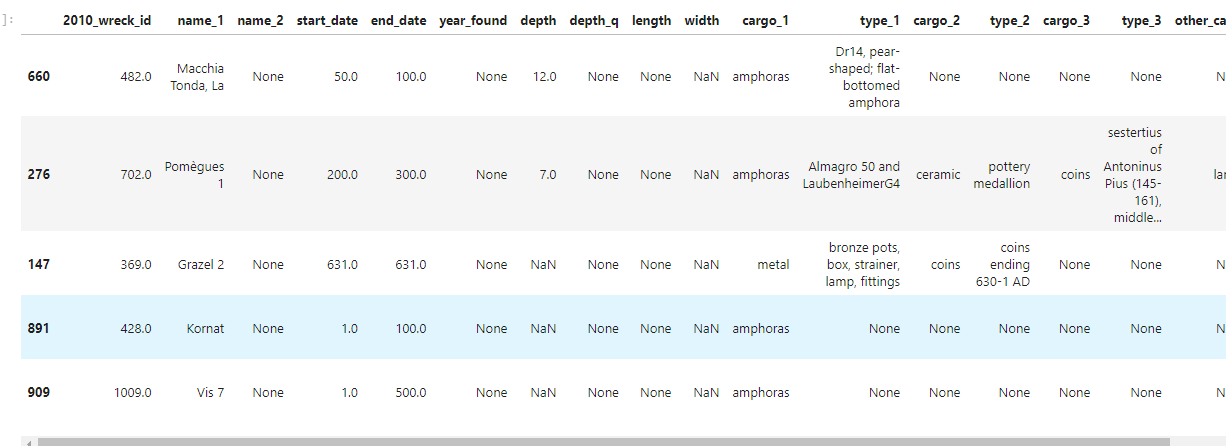
\includegraphics{./Figs/ship.png}
\end{frame}

\begin{frame}[fragile]{Vizualizimi i Pikave}
\protect\hypertarget{vizualizimi-i-pikave}{}
\AddToHookNext{env/Highlighting/begin}{\tiny}

\begin{Shaded}
\begin{Highlighting}[]
\ImportTok{import}\NormalTok{ geoplot}
\ImportTok{import}\NormalTok{ matplotlib.pyplot }\ImportTok{as}\NormalTok{ plt}

\CommentTok{\# Përkufizoni kanavacën}
\NormalTok{f, ax }\OperatorTok{=}\NormalTok{ plt.subplots(figsize}\OperatorTok{=}\NormalTok{(}\DecValTok{10}\NormalTok{,}\DecValTok{7}\NormalTok{))}

\CommentTok{\# Vizualizoni dy shtresa}
\NormalTok{countries\_df.plot(ax}\OperatorTok{=}\NormalTok{ax, color}\OperatorTok{=}\StringTok{\textquotesingle{}lightgray\textquotesingle{}}\NormalTok{, edgecolor}\OperatorTok{=}\StringTok{"none"}\NormalTok{, linewidth}\OperatorTok{=}\FloatTok{.5}\NormalTok{)}
\NormalTok{geoplot.pointplot(ship\_df, s}\OperatorTok{=}\DecValTok{2}\NormalTok{, color}\OperatorTok{=}\StringTok{\textquotesingle{}red\textquotesingle{}}\NormalTok{, ax}\OperatorTok{=}\NormalTok{ax, alpha}\OperatorTok{=}\FloatTok{.1}\NormalTok{)}

\CommentTok{\# Vendosni kufijtë e hartës}
\CommentTok{\# Krijoni një buffer për të shtuar një margjinë}
\NormalTok{buff }\OperatorTok{=}\NormalTok{ ship\_df.}\BuiltInTok{buffer}\NormalTok{(}\DecValTok{1}\NormalTok{)}
\NormalTok{xlim }\OperatorTok{=}\NormalTok{ ([buff.total\_bounds[}\DecValTok{0}\NormalTok{], buff.total\_bounds[}\DecValTok{2}\NormalTok{]])}
\NormalTok{ylim }\OperatorTok{=}\NormalTok{ ([buff.total\_bounds[}\DecValTok{1}\NormalTok{], buff.total\_bounds[}\DecValTok{3}\NormalTok{]])}
\NormalTok{ax.set\_xlim(xlim)}
\NormalTok{ax.set\_ylim(ylim)}

\CommentTok{\# Vendosni titullin e hartës}
\NormalTok{ax.set\_title(}\StringTok{\textquotesingle{}Anije të Mbytura (500 p.e.s. {-} 1500 e.s.)\textquotesingle{}}\NormalTok{)}

\CommentTok{\# Shfaqni rezultatet}
\NormalTok{plt.show()}
\end{Highlighting}
\end{Shaded}
\end{frame}

\end{document}
